\documentclass[12pt]{scrartcl}

\usepackage{booktabs}
\usepackage{amsmath,amssymb}
\usepackage{fullpage}
\usepackage{enumitem}
\usepackage{hyperref}
\usepackage{graphicx}
\usepackage{tikz}
\usepackage{pgfplots}
\usepackage{float}
\usepackage{tabularx}

\pgfplotsset{compat=1.18}
\usetikzlibrary{trees,positioning,shapes,arrows}
\usepgfplotslibrary{statistics} 
\setlength{\parindent}{0pt}

\tikzset{
  basic/.style  = {draw, text width=2cm, drop shadow, font=\sffamily, rectangle},
  root/.style   = {basic, rounded corners=2pt, thin, align=center, fill=white},
  level-2/.style = {basic, rounded corners=6pt, thin,align=center, fill=white, text width=3cm},
  level-3/.style = {basic, thin, align=center, fill=white, text width=1.8cm}
}


\begin{document}

\begin{center}
	\hrule
	\vspace{0.4cm}
	{\textbf{\large Lecture 1: Descriptive Statistics}}\\ [0.2cm]
	INF1004 Mathematics II

\end{center}

\textbf{Name:} Timothy Chia \hspace{\fill} \textbf{Date:} 05/01/2025 \\

\hrule

\begin{enumerate}[label=\textbf{\arabic*.}]

	\item \textbf{What is Statistics?}

	      Statistics is the art of collecting, analysing, and interpreting data. It allows us to discover hidden patterns and make informed decisions, even when we face uncertainty in the real world.

	      \medskip

	      Broadly, statistics can be divided into three closely related areas:

	      \medskip

	      \begin{table}[htbp]
		      \centering
		      \begin{tabularx}{\linewidth}{@{}X X X@{}}
			      \toprule
			      \textbf{Descriptive Statistics} & \textbf{Probability Theory} & \textbf{Inferential Statistics} \\
			      \midrule
			      This branch involves collecting, organising, summarising, and presenting the data you actually have.
			                                      &
			      This branch links descriptive statistics to inferential statistics by focusing on modelling randomness and uncertainty using mathematical frameworks.
			                                      &
			      This branch involves making predictions, testing hypotheses, and drawing conclusions about a population based on a smaller sample.
			      \\
			      \bottomrule
		      \end{tabularx}
	      \end{table}

	      \medskip

	      \textbf{Data Sources}

	      \begin{itemize}
		      \item \textbf{Population:} The entire collection of all individuals or items of interest. Measuring every single item in a population is called a \emph{census}, which is often expensive and time-consuming.
		      \item \textbf{Sample:} A smaller subset selected from the population. We study the sample to estimate properties of the population. The process of selecting this subset is called \emph{sampling}.
	      \end{itemize}

	      \medskip

	      To describe populations and samples more precisely, we can use simple mathematical notation.

	      \medskip

	      \textbf{Definitions}

	      Let $P$ be the sample space of a particular population being investigated.
	      Let $S$ be a sample drawn from the population such that $S \subset P$.


	      \newpage
	\item \textbf{Types of Data}

	      \vspace{0.8\baselineskip}

	      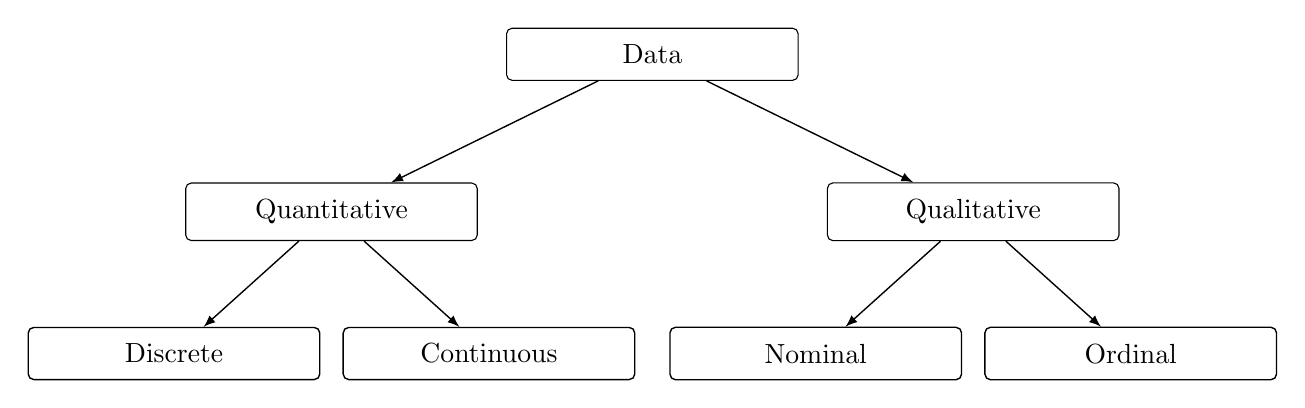
\begin{tikzpicture}[
			      grow=down,
			      level 1/.style={sibling distance=8.15cm, level distance=20mm},
			      level 2/.style={sibling distance=4cm, level distance=18mm},
			      edge from parent/.style={draw, -latex, line width=0.5pt},
			      every node/.style={font=\normalsize},
			      box/.style={
					      draw,
					      rounded corners=2pt,
					      align=center,
					      inner xsep=10pt,
					      inner ysep=6pt,
					      text width=3.0cm
				      }
		      ]
		      \node[box]{Data}
		      child {
				      node[box]{Quantitative}
				      child { node[box]{Discrete} }
				      child { node[box]{Continuous} }
			      }
		      child {
				      node[box]{Qualitative}
				      child { node[box]{Nominal} }
				      child { node[box]{Ordinal} }
			      };
	      \end{tikzpicture}

	      \vspace{1.0\baselineskip}

	      \begin{itemize}
		      \setlength{\itemsep}{10pt}
		      \setlength{\topsep}{6pt}
		      \setlength{\parsep}{2pt}

		      \item \textbf{Quantitative (Numeric):} Expresses numeric data and represents amounts or quantities.
		            \begin{itemize}
			            \setlength{\itemsep}{6pt}
			            \setlength{\topsep}{4pt}
			            \item \textbf{Discrete:} Numeric data that are specific, countable values.
			            \item \textbf{Continuous:} Numeric data that can take any value within a range such that it can be measured with increasing precision.
			                  % \item \emph{Example:} Height, time taken to complete a task, income.
		            \end{itemize}

		            \vspace{0.4\baselineskip}

		      \item \textbf{Qualitative (Categorical):} Expresses non-numeric data and generally represents some quality, characteristic, or category.
		            \begin{itemize}
			            \setlength{\itemsep}{6pt}
			            \setlength{\topsep}{4pt}
			            \item \textbf{Nominal:} Categories that are just names or labels with no inherent order or ranking.
			                  % \item \emph{Example:} Eye colour, race, yes/no answers.
			            \item \textbf{Ordinal:} Categories that have a meaningful order or ranking, but the difference between the ranks is not necessarily equal.
			                  % \item \emph{Example:} Satisfaction ratings (Unhappy $\to$ Neutral $\to$ Happy), T-shirt sizes (S, M, L).
		            \end{itemize}
	      \end{itemize}

	      %------------------------------------------------------------
	      \newpage
	\item \textbf{Graphical Presentation of Data}

	      \textbf{Categorical Data:}
	      \begin{itemize}
		      \item \textbf{Frequency Table:} A simple summary that lists each category alongside its frequency ($f_i$, the count) or relative frequency ($p_i = f_i / N$, the proportion).
		      \item \textbf{Graphical:}
		            \begin{itemize}
			            \item \textbf{Bar Charts:} Use separate bars (with gaps between them) to compare different categories.
			            \item \textbf{Pie Charts:} Show how a whole is divided into different categories (best for showing proportions).
		            \end{itemize}
	      \end{itemize}

	      \medskip

	      \textbf{Quantitative Data:}
	      \begin{itemize}
		      \item \textbf{Frequency Distribution:} Because numeric data can be vast, we group it into "classes" or "intervals" to see the pattern.
		      \item \textbf{Histogram:} The most common way to visualize numeric distributions. Unlike bar charts, the bars in a histogram \emph{touch each other} to indicate that the data is continuous number-line data.
		      \item \textbf{Unequal Class Widths:} Sometimes, grouping intervals have different sizes. If we simply plotted frequency, wider bars would look visually "heavier" or more important than they should. To correct this, we use \textbf{Density} for the height.
		            \[
			            \text{Density} = \frac{\text{Relative Frequency}}{\text{Class Width}}
		            \]
		            \emph{Note:} In a density histogram, the \emph{area} of the bar represents the frequency, not just the height.
	      \end{itemize}

	      \medskip

	      \textbf{Bivariate Data (Two Variables):}
	      \begin{itemize}
		      \item \textbf{Crosstabulation (Contingency Table):} A table that displays the frequency distribution of two variables simultaneously (e.g., "Gender" vs. "Subject Choice").
		      \item \textbf{Charts:} \textbf{Stacked} or \textbf{Clustered Bar Charts} allow you to compare sub-groups within the data side-by-side.
	      \end{itemize}

	      %------------------------------------------------------------
	      \newpage
	\item \textbf{Measures of Central Tendency}

	      Data may be presented numerically to succinctly describe it. There are three basic measures – central tendency (or position), spread and relative standing.

	      \medskip

	      \textbf{Mean Definition}

	      Let $x_1,x_2,\dots,x_m$ be a collection of $m$ numerical observations. The mean of these observations is defined as
	      $$\frac{1}{m} \sum_{i=1}^{m}x_i$$

	      If the observations constitute the entire population of size $N$, the mean is called the \textbf{population mean} and is denoted by $\mu$, where
	      $$\mu = \frac{1}{N} \sum_{i=1}^{N}x_i$$

	      If the observations form a sample of size $n$ drawn from the population, the mean is called the \textbf{sample mean} and is denoted by $\bar{x}$, where
	      $$\bar{x} = \frac{1}{n} \sum_{i=1}^{n}x_i$$

	      Here, $N$ denotes the population size, $n$ denotes the sample size with $n<N$, and the distinction between $\mu$ and $\bar{x}$ reflects whether the mean is taken over the full population or over a sample.

	      \medskip

	      \textbf{Median Definition}

	      Let $x_1, x_2, \ldots, x_m$ be a collection of $m$ numerical observations arranged in non-decreasing order. The \textbf{median} is defined as the central value of the ordered data.

	      \begin{itemize}
		      \item If $m$ is odd, the median is the value in position $\frac{m+1}{2}$.
		      \item If $m$ is even, the median is defined as the arithmetic mean of the values in positions $\frac{m}{2}$ and $\frac{m}{2+1}$.
	      \end{itemize}

	      \medskip

	      \textbf{Mode Definition}

	      The \textbf{mode} is defined as the value(s) that occur with the greatest frequency in the data set. A data set may have no mode if all values occur with equal frequency, one mode if a single value occurs most frequently, or multiple modes if several values share the highest frequency.

	      %------------------------------------------------------------
	      \newpage
	      \textbf{Histogram Skewness}

	      \begin{figure}[htbp]
		      \centering
		      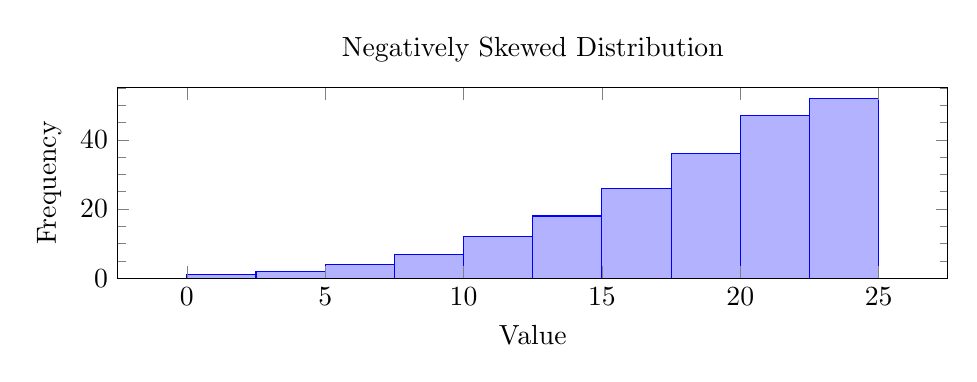
\begin{tikzpicture}
			      \begin{axis}[
					      width=\linewidth,
					      height=4cm,
					      ymin=0, ymax=55,
					      minor y tick num=3,
					      area style,
					      title={Negatively Skewed Distribution},
					      xlabel={Value},
					      ylabel={Frequency},
					      xtick={0,5,10,15,20,25},
				      ]
				      \addplot+[ybar interval, mark=no] plot coordinates {
						      (0,  1) (2.5, 2) (5,  4) (7.5, 7) (10, 12)
						      (12.5,18) (15, 26) (17.5,36) (20, 47) (22.5,52) (25, 0)
					      };
			      \end{axis}
		      \end{tikzpicture}
		      \caption{A negatively (left) skewed distribution with a long tail towards smaller values; $mean < median < mode$.}
		      \label{fig:negative-skew}
	      \end{figure}

	      \begin{figure}[htbp]
		      \centering
		      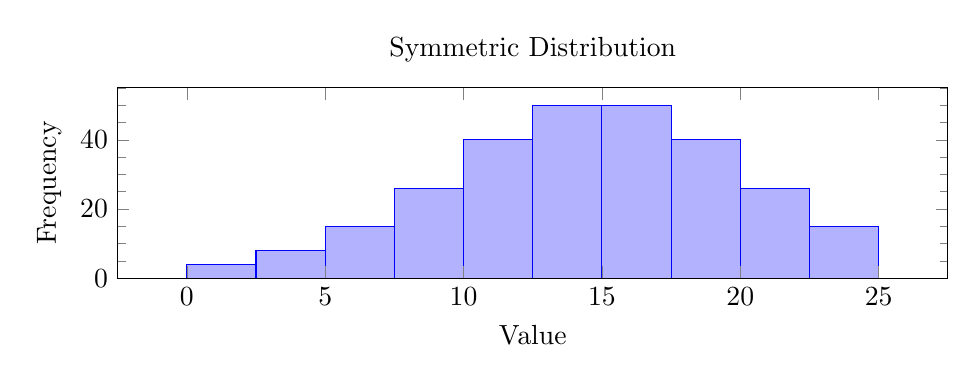
\begin{tikzpicture}
			      \begin{axis}[
					      width=\linewidth,
					      height=4cm,
					      ymin=0, ymax=55,
					      minor y tick num=3,
					      area style,
					      title={Symmetric Distribution},
					      xlabel={Value},
					      ylabel={Frequency},
					      xtick={0,5,10,15,20,25},
				      ]
				      \addplot+[ybar interval, mark=no] plot coordinates {
						      (0,  4) (2.5, 8) (5,  15) (7.5, 26) (10, 40)
						      (12.5,50) (15, 50) (17.5,40) (20, 26) (22.5,15) (25, 0)
					      };
			      \end{axis}
		      \end{tikzpicture}
		      \caption{An approximately symmetric distribution with no pronounced tail;\\ $mean = median = mode$.}
		      \label{fig:symmetric}
	      \end{figure}

	      \begin{figure}[H]
		      \centering
		      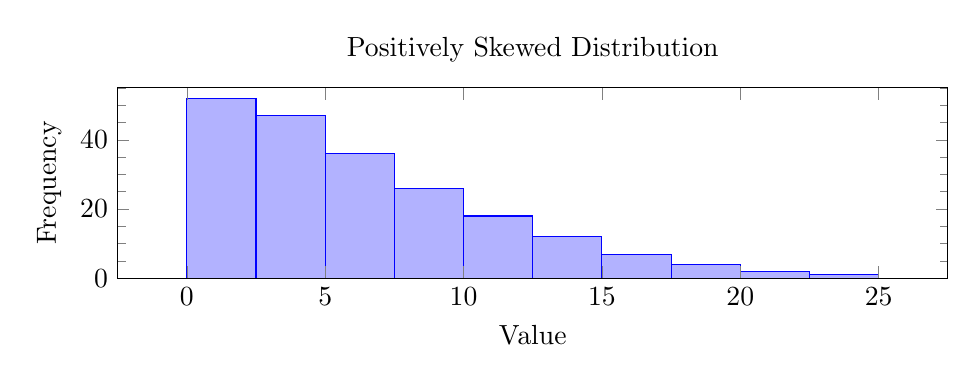
\begin{tikzpicture}
			      \begin{axis}[
					      width=\linewidth,
					      height=4cm,
					      ymin=0, ymax=55,
					      minor y tick num=3,
					      area style,
					      title={Positively Skewed Distribution},
					      xlabel={Value},
					      ylabel={Frequency},
					      xtick={0,5,10,15,20,25},
				      ]
				      \addplot+[ybar interval, mark=no] plot coordinates {
						      (0,  52) (2.5,47) (5,  36) (7.5,26) (10, 18)
						      (12.5,12) (15, 7) (17.5, 4) (20, 2) (22.5, 1) (25, 0)
					      };
			      \end{axis}
		      \end{tikzpicture}
		      \caption{A positively (right) skewed distribution with a long tail towards larger values; $mean > median > mode$.}
		      \label{fig:positive-skew}
	      \end{figure}





	      % positive skew - mean > median\\
	      % no skew - mean = median\\
	      % negative skew - mean < median\\

	      % \textbf{Histogram Modality}
	      % describes the number of peaks in a histogram.

	      % unimodal - one peak\\
	      % bimodal - two peaks\\
	      % trimodal - three peaks\\
	      % and so on.\\

	      %------------------------------------------------------------
	      \newpage
	\item \textbf{Measures of Relative Standing}

	      Measures of relative standing describe the position of an observation relative to the other values in a dataset, rather than its absolute size. Common measures include quartiles and percentiles.

	      \medskip

	      \textbf{Quartiles:}
	      Quartiles divide an ordered dataset into four equal parts (quarters). Each part contains 25\% of the data.
	      \begin{itemize}
		      \item $Q_1$ (Lower Quartile): the value below which 25\% of the data lie
		      \item $Q_2$ (Median): the value below which 50\% of the data lie
		      \item $Q_3$ (Upper Quartile): the value below which 75\% of the data lie
	      \end{itemize}

	      \medskip

	      \textbf{Percentiles:}
	      Percentiles generalise the idea of quartiles. The $p$th percentile is the value below which $p\%$ of the data lie.
	      For example, the 90th percentile is the value below which 90\% of observations fall.

	      \medskip

	      \textbf{Box-and-Whisker Plot:}
	      Quartiles and the overall distribution of the data are commonly visualised using a box-and-whisker plot.
	      \begin{itemize}
		      \item The box spans from $Q_1$ to $Q_3$ and represents the interquartile range (IQR)
		      \item The line inside the box marks the median ($Q_2$)
		      \item The whiskers extend to the smallest and largest non-outlier values
		      \item Points beyond the whiskers (if shown) represent outliers
	      \end{itemize}

	      \medskip

	      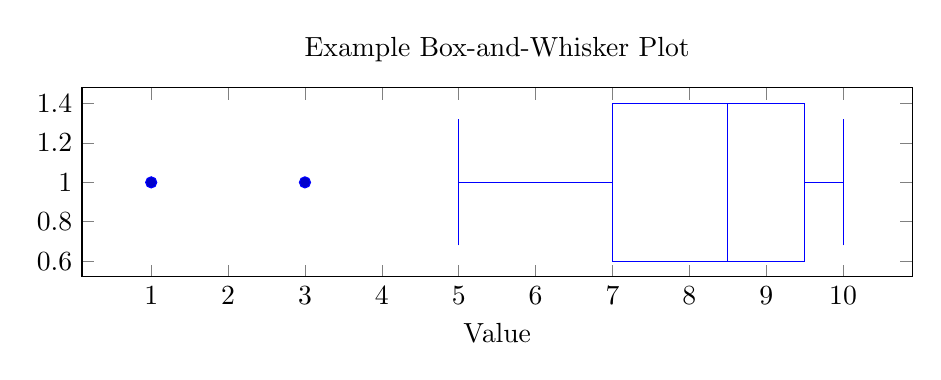
\begin{tikzpicture}
		      \begin{axis}[
				      width=\linewidth,
				      height=4cm,
				      y=2.5cm,
				      xlabel={Value},
				      title={Example Box-and-Whisker Plot},
			      ]
			      \addplot+[
				      boxplot prepared={
						      lower whisker=5,
						      lower quartile=7,
						      median=8.5,
						      upper quartile=9.5,
						      upper whisker=10,
					      },
			      ]
			      table [row sep=\\, y index=0] {
					      data\\ 1\\ 3\\
				      };
		      \end{axis}
	      \end{tikzpicture}

	      \medskip

	      From the boxplot, we can quickly identify the median, the spread of the middle 50\% of the data, and whether the distribution appears symmetric or skewed.

	      %------------------------------------------------------------
	      \newpage
	\item \textbf{Measures of Spread}

	      Measures of spread (also called measures of dispersion) describe how variable or spread out a dataset is around its centre.

	      \medskip

	      \textbf{Range:}
	      The simplest measure of spread. It only considers the extreme values in the dataset and is therefore highly susceptible to outliers. It also ignores all values between the minimum and maximum.
	      \[
		      \text{Range} = \text{Highest Value} - \text{Lowest Value}
	      \]

	      \medskip

	      \textbf{Interquartile Range (IQR):}
	      Measures the spread of the middle 50\% of the data after the data have been ordered. Because it ignores the extremes, it is a robust measure of spread.
	      \[
		      \text{IQR} = Q_3 - Q_1
	      \]
	      \begin{itemize}
		      \item \textbf{Outliers:} The IQR is commonly used to identify unusual values. A data point is considered an outlier if it lies below $Q_1 - 1.5(\text{IQR})$ or above $Q_3 + 1.5(\text{IQR})$. This rule is a convention rather than a strict mathematical law.
	      \end{itemize}

	      \medskip

	      \textbf{Variance ($s^2$):}
	      Ideally, we want to measure the average distance of data points from the mean. Variance does this by calculating the average \emph{squared} distance from the mean, where squaring ensures all values are positive. A larger variance indicates greater dispersion around the mean.
	      \begin{itemize}
		      \item \textbf{Sample Variance Formula:} We divide by $n-1$ instead of $n$ to obtain a better estimate of the population variance. This adjustment is known as Bessel's correction.
		            \[
			            s^2 = \frac{\sum (x_i - \bar{x})^2}{n-1}
		            \]
		      \item \textbf{Alternative Formula (Computational):} A mathematically equivalent formula often used in manual calculations to reduce rounding errors.
		            \[
			            s^2 = \frac{1}{n-1} \left[ \sum x_i^2 - \frac{(\sum x_i)^2}{n} \right]
		            \]
	      \end{itemize}

	      \medskip

	      \textbf{Standard Deviation ($s$):}
	      Because variance is measured in squared units (for example, dollars squared), it can be difficult to interpret. Taking the square root returns the measure to the original units of the data.
	      \[
		      s = \sqrt{s^2}
	      \]

	      \medskip

	      \textbf{Coefficient of Variation (CV):}
	      Standard deviation is an absolute measure of spread. The coefficient of variation is a \emph{relative} measure, expressed as a percentage. It is particularly useful for comparing variability or risk between datasets with very different means. However, it should not be used when the mean is close to zero.
	      \[
		      CV = \frac{s}{\bar{x}} \times 100\%
	      \]


\end{enumerate}

\end{document}


